
% This is samplepaper.tex, a sample chapter demonstrating the
% LLNCS macro package for Springer Computer Science proceedings;
% Version 2.20 of 2017/10/04
%
\documentclass[runningheads]{llncs}
%
\usepackage{graphicx}
\usepackage{hyperref}
\renewcommand\UrlFont{\color{blue}\rmfamily}
\setlength{\parskip}{0pt}
\raggedbottom

\usepackage{amsmath}
\usepackage{csquotes}
\usepackage{paralist}
\usepackage{booktabs}
\usepackage{mathptmx}
\usepackage{pgfplots}
\pgfplotsset{compat=1.8}
\usepackage{subfigure}

\begin{document}
%
\title{VERS UN MODELE DE PREVISON EFFICACE DES CAS DE PALUDISME AU SENEGAL}
%
%\titlerunning{Abbreviated paper title}
% If the paper title is too long for the running head, you can set
% an abbreviated paper title here
%
\author{Ousseynou Mbaye \and Mouhamadou Lamine Ba \\ Gaoussou Camara \and Alassane Sy}
%
\authorrunning{Ousseynou Mbaye \and M. Lamine Ba \and Gaoussou Camara \and Alassane Sy}
% First names are abbreviated in the running head.
% If there are more than two authors, 'et al.' is used.
%
\institute{Universit\'e Alioune Diop de Bambey, Bambey, Senegal\\
\email{firstmidlle.last@uadb.edu.sn}
%\email{ousseynou.mbaye@uadb.edu.sn}\\
%\email{mouhamadoulamine.ba@uadb.edu.sn}\\
%\email{gaoussou.camara@uadb.edu.sn}\\
%\email{alassane.sy@uadb.edu.sn}
}
%
\maketitle              % typeset the header of the contribution
%
\begin{abstract}
Le paludisme est l’une des maladies les plus mortelles dans le monde plus particulièrement en Afrique subsaharien. La situation est critique dans des pays comme le Senegal à cause du manque de services de santé  de qualité et de personnel médical qualifie et capable de faire des diagnostics précis des maladies dont souffrent les patients.
Ainsi la nécessité de trouver des outils automatisées pour aider les acteurs médicaux dans le processus de prise de décision après avoir réalisé le diagnostic.
Dans ce papier nous proposons les premières étapes vers la réalisation d’un algorithme de diagnostic du paludisme basé sur les signes et symptômes du patient en plus du TDR (Test de Diagnostic Rapide). Notre modèle de prédiction est basée sur la régression logistique.
Les résultats des premiers tests sur un jeu de données  réel et semi-synthétique de patients se sont très prometteurs concernant l’efficacité de l’approche proposée.

 Mots clés : Diagnostic, Paludisme, Modèle de Prédiction, Imputation des données

\end{abstract}
%
%
% Introduction
\section{Introduction}\label{intro}
% context and motivations

Malaria is one amongst the most deadly disease in the world, especially in sub-saharan Africa countries such as Senegal.
Malaria is caused by parasitic single-celled microorganisms belonging to the Plasmodium group; it is an infectious
disease which is transmitted to human being through bites from infected female Anopheles mosquitoes. Someone who suffers
from  Malaria may present symptoms that typically include fever, tiredness, vomiting, and headaches. In its severe form,
the disease can cause yellow skin, seizures, coma or death.

According to the last report about the propagation of Malaria disease around the world, published in November 2017, 216 millions of cases have been 
reported in 2016. As a result, the number of cases has significantly increased when compared to the 211 millions of reported Malaria patients in 2016.
As for the number of death due to Malaria, it does not decrease between 2016 and 2017 (446.000 vs. 445.000) despite the huge effort made by governements
and non-governmental organization to improve healthcare services and the awareness strategies, especially in critical areas. 
When analyzing the statistics above in details, one can easily notice that the burden of the Africa region of the World 
international Health Organization (WHO in short) is colossal. Indeed, 90\% of Malaria cases and 90\% of deaths due to the disease were located in this area in 2016.
More specifically, 80\% of the burden in terms of morbidity is distributed in fifteen countries, all located in Sub-saharan Africa except India. This demonstrates
that Malaria is a real flail in Sub-saharan Africa states and Senegal is not spared at all.

  


% studied problem and proposed solution










% Papier organization

\paragraph*{Paper organization.}The remaining of the paper is organized as follows. We summarize the related work on data imputation and binary classification methods in Section \ref{related_work}.
In Section \ref{data_prep} we introduce the data profiling and imputation techniques used on patient records. We then present our prediction model for Malaria cases in Section \ref{prediction_model}.
Experimentation on real-world datasets are detailled in Section \ref{experimentation} before we conclude in Section \ref{conclusion}. 


% Related work
\section{Revue de la littérature}\label{Revue de la littérature}
Dans cette section, nous résumons l’état de la recherche sur le paludisme en général, et en particulier l’utilisation des techniques d’apprentissage automatique pour aborder les différents aspects liés à l’un des principaux problèmes de santé dans le monde, notamment le paludisme
Comme on le sait bien, le paludisme est causé par la piqure de l’anophèle femelle, dont la plus dangereuse espèce est le Plasmodium falciparum. De nombreux travaux préliminaires ont été ensuite consacrés à l’étude de l’évolution et de la répartition du moustique responsable, principalement dans le but de détecter ou de diagnostiquer la gravité de la maladie par rapport à un patient infecté donné [10 , 5]. Les recherches récentes sur le paludisme ont largement adopté le machine learning et ont démontré sa capacité à résoudre divers aspects de la maladie. La plupart de ces techniques basées sur le machine learning reposent sur l'analyse des données sanguines obtenues à partir de captures d'écran microscopiques de haute définition comme dans [12 ]. Les auteurs dans [12] proposent un algorithme d'apprentissage non supervisé qui détecte et détermine les types de cellules sanguines infectées. L’approche de prédiction utilisée consiste à quantifier la quantité de parasite plasmodium dans un frottis sanguin. Dans la même intuition de recherche d’exploitation du sang. ‘The Jordan-Elman neural networks classifier’ introduit dans [ 7] ,permet rapidement déterminer l'occurrence du paludisme et son niveau de gravité également. Elle est basée sur une analyse des caractéristiques des données sanguine des patients par le réseau de neurones. Toujours en utilisant le machine learning, DIAZ et al. ont proposé dans [ 9] un algorithme semi-supervisé permettant de quantifier et de classer les érythrocytes infectés par les parasites du paludisme à travers des images microscopiques. L'originalité de cette méthode vient de son efficacité même en présence de fines pellicules de sang infecté par le Plasmodium falciparum pour la quantification et de classification des parasites plasmodium infectés. Outre les données sanguines, des enregistrements de signes et de symptômes des patients ont également été utilisés pour étudier le paludisme avec les méthodes  de machine learning. En effet, une approche basée sur les arbres de décision a été proposée au Nigeria [ 23] pour prédire la survenue du paludisme à partir des données de diagnostic. Cependant, un arbre de décision souffre de diverse limite en tant que classificateur. En effet, il peut facilement sur-adapter ou peut être extrêmement sensible aux petites variations dans les données. Quand bien même nous nous appuyons et sur les signes et sur les symptômes, le modèle de prédiction dans [ 23] diffère du nôtre sur de nombreuses facettes: notre modèle est construit sur la régression logistique et est entrainé  en utilisant également les informations du test de diagnostic rapide. De plus, nous appliquons notre méthode dans le contexte de patients vivant au Sénégal. Un exemple du travail cité précédemment et qui a utilisé la régression logistique est celui de Farida et al. dans [ 3]. La régression logistique y est utilisée pour la sélection des attributs afin de construire des arbres de décision stables. Les arbres de décision sont ensuite utilisés pour prédire les critères de gravité du paludisme dans le contexte afghan.
Dans la lignée des travaux appliquant l’apprentissage automatique, dans [ 16] , Pranav et al. proposent un agent d'apprentissage par Reinforcement Learning  (RL) capable de prédire la probabilité qu'un individu présente un résultat positif au test du paludisme en posant des questions sur leur ménage. Cet agent est un Deep Q-network  RL qui apprend une politique directement à partir des réponses aux questions, avec une action définie pour chaque question de sondage possible et pour chaque classe de prédiction possible. En outre, une classification fondée sur des règles statistiques  améliorées et permettant de diagnostiquer le paludisme a été proposé dans [6].Un prototype correspondant intégrant les règles et les modèles statistiques a été mis en place; L’objectif principal de l’étude était de développer un prototype statistique permettant de réaliser un diagnostic clinique du paludisme, compte tenu de ses effets indésirables sur l’ensemble des soins de santé. Toutefois, son traitement reste très coûteux pour la majorité des patients.
À notre connaissance, il s’agit du premier travail au Sénégal qui tente de fournir un modèle de prédiction du paludisme à partir des données des patients.



% Data Preparation
\section{Traitement des données}\label{Traitement des données}
Dans cette section, nous détaillons le processus de préparation des données suivi pour l’obtention d’un jeu de données sur le paludisme pour la phase de prédiction. Nous commençons par présenter les techniques de nettoyages et de normalisation des données utilisées.
\subsection{Nettoyage et labélisation des données}
Dans le but de mettre en place un modèle de prédiction efficace des cas de paludisme au Sénégal, nous nous sommes appuyés sur un jeu de données de patients réel pour la validation. Le jeu de données a été extrait du Grand Magal de Touba de 2016 [19 ]. Environ 4-5 millions d'individus se réunissent chaque année dans la ville sainte de Touba, au Sénégal, lors de la cérémonie religieuse du Grand Magal. Plusieurs points de santé sont établis lors de cet événement religieux; chaque point reçoit chaque jour des centaines de patients, dont certains atteints de paludisme. Les données de patients que nous utilisons ici ont été recueillies manuellement à partir des registres de ces points puisqu’ aucun système de gestion électronique de la santé n’existe. En détail, l’ensemble des données comprend des milliers d’enregistrements de patients comportant chacun 16 caractéristiques. Certaines de ces caractéristiques (également appelées fonctionnalités) comprennent des données personnelles sur le patient, mais aussi les signes et les symptômes du patient signalés par le médecin qui a pris le patient en charge. Les autres attributs décrivent des données cliniques telles que des informations sur le diagnostic final du médecin (la maladie dont souffre le patient), le résultat du test de diagnostic rapide (TDR) et le statut (c.-à-d. admission, décédé ou mis sous observation) du patient. Pour des raisons de confidentialité et certaines restrictions d’utilisation des données, nous avons ignoré les données personnelles sur le patient pendant ce travail. En raison du fait que les données des patients ont été collectées manuellement dans des registres, nous avons constaté de nombreuses incohérences telles que fautes d'orthographe, mêmes valeurs d'attributs avec des écritures différentes (par exemple, «DIARRHEE INFECTIEUSE ”et“ INFECTIEUSE DIARRHE ”), et des attributs à valeurs multiples (par exemple la colonne signes et symptôme). Nous utilisons le logiciel OpenRefine [13 , 1] pour d’abord nettoyer  puis normaliser les valeurs dans l'ensemble des données  des patients. OpenRefine (Google raffiné) est un puissant outil open source qui permet aux chercheurs ou aux scientifiques d’accomplir l’activité de criblage des données, c’est-à-dire  de travailler avec des données en désordre: les nettoyer; les transformer d'un format à un autre; et les compléter avec des services Web et des données externes. Nous avons utilisé les méthodes suivantes fournies par OpenRefine pour prétraiter notre jeu de données brutes.
\begin{itemize}
\item \textbf{Text filter function:} le filtre de texte permet d’explorer les valeurs des attributs, de les nettoyer et d’identifier ceux qui peuvent avoir de nombreuses variantes.
\item \textbf{Transform functions:} OpenRefine fournit deux fonctions de transformation différentes: les fonctions de transformations prédéfinies (preset transformations functions) pour la résolution de problèmes de mise en forme triviaux tels que le rognage des espace blancs et des fonctions de transformations avancées (Advanced transformations) basées sur le langage (GREL) de OpenRefine pour normaliser les données par lots ou les fractionner. Cette deuxième classe de formations est très utile, en particulier lorsque le nombre de valeurs de données à normaliser est très important (faire la même tâche manuellement prendrait beaucoup de temps et serait sujette aux erreurs). Par exemple, GREL permet d’utiliser une expression régulière simple pour toutes les variantes d'un symptôme dans la colonne Symptôme.
\item \textbf{Cluster and edit function:} l'option de groupage dans OpenRefine fournit également aux utilisateurs des méthodes pour fusionner et normaliser les variations dans l'ensemble de données. La puissance de cette fonction est qu'il est capable de détecter automatiquement les petites variations de données qui suivent un certain modèle.
\end{itemize}
En ce qui concerne le cas particulier des attributs à valeurs multiples tels que les colonnes symptôme et diagnostic de notre jeu de données brutes, nous les avons divisés en plusieurs valeurs dans des colonnes distinctes. En effet, dans le jeu de données brutes, des informations telles que les symptômes dont un patient donné souffre ont été stockés dans une seule colonne, séparée par le caractère spécial '+', par exemple \textquote{DOULEUR ARTICULAIRE}+\textquote{DOULEUR PELVIENNE} +\textquote{VOMISSEMENTS}.
Après cette étape de nettoyage et de normalisation des données, nous avons procédé à l'extraction des caractéristiques du paludisme.
\subsection{Sélection  des caractéristiques du paludisme}
Pour bien étudier le paludisme, il faut disposer d’un ensemble de données d’un  patient comprenant les principales caractéristiques de la maladie.  Malheureusement, certaines de ces caractéristiques du paludisme n’étaient pas explicitement spécifiées dans notre jeu de données brutes. En conséquence, nous avons déduit douze nouveaux attributs qui décrivent mieux les signes et les symptômes du paludisme selon les experts du monde de la santé. Ces nouveaux attributs sont: \emph{manque d’appétit}, \emph{fatigue}, \emph{fièvre}, \emph{céphalalgie}, \emph{nausée}, \emph{arthralgie}, \emph{troubles digestifs}, \emph{vertiges}, \emph{frissons}, \emph{myalgie}, \emph{diarrhée} et \emph{douleurs abdominales}. Nous avons ensuite ajouté les nouveaux attributs à notre jeu de données et transformé ce dernière en remplissant la valeur de chaque nouvel attribut en fonction de la liste des signes et des symptômes signalés pour chaque patient.
Le Diagnostic est le résultat des signes et symptômes confirmé par un examen médical en général. Dans la colonne Diagnostic, on voit plusieurs conclusions différentes. Ainsi tout diagnostic autre que le paludisme est remplacé par la classe non paludisme
À cette étape de notre processus de préparation de données, nous avons créé un jeu de données patient contenant les caractéristiques requises pour le paludisme. Cependant, notre jeu de données n'était pas encore complet ni prêt à cause de l'absence de valeurs. Enfin, nous avons complété notre ensemble de données en utilisant une approche d’imputation des données robuste
\subsection{ Imputation de données manquantes}
Comme le montre le tableau\ref{table-missing}, nous avons observé de nombreuses valeurs manquantes dans notre jeu de données, affectant ainsi la majorité des attributs de données. Ces valeurs manquantes ne doivent pas être ignorées car les données d’autant plus que l'exhaustivité et la qualité sont très importantes pour traiter un problème de prédiction; ceci pourrait avoir un impact négatif sur la précision de nos prédictions et devrait être traité de manière appropriée. Il faut noter que l'apprentissage automatique repose sur un ensemble de données complet. Les sources et les types de valeurs manquantes peuvent être variés\cite{Al18}. Dans notre contexte, les manquements ne sont pas \emph{complètement aléatoires} et peuvent être dus à une connaissance incomplète des données du patient, au fait que le personnel médical ne spécifie pas une valeur d’attribut lorsqu’elle n’est pas observée, ou à une difficulté pour les patients à décrire correctement certaines informations (liées par exemple aux signes ou aux symptômes de leurs maladies) au moment du diagnostic. Puisqu'ils pourraient avoir une certaine relation entre les valeurs d'attribut pour le même patient, voire une corrélation entre les dossiers des patients, nous décidons de résoudre notre problème de valeurs manquantes en utilisant des algorithmes d'imputation au lieu de choisir des valeurs arbitraires ou de supprimer des enregistrements avec valeurs manquantes.
L’imputation des données est souvent utilisée dans le domaine de l’apprentissage automatique pour traiter les erreurs d’informations. De nombreux algorithmes ont été proposés dans la littératuret \cite{Si14,Al18}, dépendant de la nature de l’absence ou du type de données. MissForest\cite{Ste12}a été prouvé très efficace en présence de divers types de données simultanément comme dans notre cas (par exemple données numériques, chaîne, données catégorielles, etc.). L'algorithme missForest s'appuie sur 
RandomForest qui est une méthode de prédiction non paramétrique capable de traiter des données mixtes et qui permet des effets de régression interactifs et non linéaires. Un tel algorithme d’imputation vise à traiter tous jeu de données d’information en minimisant (dans la mesure du possible) les présomptions sur les aspects structurels des données. Étant donné un ensemble de données d’information, missForest résout le problème de données manquantes en utilisant un schéma d'imputation itérative aléatoire sur les valeurs observées dans une première étape, suivie de la prédiction des valeurs manquantes puis procédant de manière itérative jusqu'à la convergence.
Nous avons appliqué missForest à notre jeu de données de patient du paludisme obtenu du paludisme précédemment  en utilisant le logiciel Python \cite{MF_python}. 
Nous étudierons et prouverons dans la section 5\ref{Expérimentation et Résultats} précisions de la prédiction faite par l’algorithme à l’aide la NRMSE (normalized root mean squared Error).

% table of the number of missing values per attribute
\begin{table}[!ht]
\centering
\begin{tabular}{cc}
\textbf{Attribute name} & \textbf{\#missing\_values}\\
\toprule
Lack of appetite &    21068 \\
digestive disorders & 21062 \\
Loss of weight &   21017 \\
Arthragia &     20940\\
Chill &      20925\\
Nausea &     20874\\
Myalgia &    20870\\
Tiredness&   20713 \\
Diarrhea &     20481\\
Vomit &        20051 \\
Abdominal pain &  19770 \\
Dizziness &       19628 \\
Fever &        18245 \\
Temperature &     17636 \\
Arterial pressure &    16924 \\
Cephalalgia &       15370 \\
Diagnostic  &     2875 \\
Quick diagnostic test &  76 \\
\bottomrule
\end{tabular}
\vspace*{.5cm}
\caption{The number of missing values per attribute}\label{table-missing}
\end{table} 



% Prediction Model
\section{Modèle de Prédiction}\label{Modèle de Prédiction}
Pour prédire le paludisme à partir du jeu de données labélisé obtenue étant donné un nouveau patient, nous utilisons la régression logistique comme \emph{prédicteur}. Dans cette section, nous rappelons brièvement les bases de la fonction de régression logistique. Puisque notre problème est un problème de classification binaire, nous commençons par introduire le problème de classification binaire que nous devons résoudre dans l'étude.
\subsection{Classification Binaire}
Supposons deux classes de diagnostic du paludisme: le \emph{paludisme} et le \emph{non-paludisme}. Nous considérons également \textsc{P} et \textsc{C} comme l’ensemble des patients et un modèle de prédiction. Un patient dans \emph{p} in \textsc{P} est défini par un ensemble de paires $(a_1, v_1), (a_2, v_2), \ldots, (a_n, v_n)$  $a_i$ et $v_i$, pour chaque $1\leq i\leq n$, correspond respectivement à une caractéristique donnée du paludisme et à sa valeur numérique associée définie comme suit.
        
\begin{equation}
v_i = \left\{
\begin{array}{rl}
1 &\text{if $a_i$ is observed} \\
0 &\text{otherwise} \\
\end{array}
\right.
\end{equation}
\begin{definition}{(Notre problème de prédiction)}  Nous définissons notre problème de classification binaire pour la prédiction de la présence ou non du paludisme sur un jeu  de données de patients donné, comme une fonction \textsc{C} qui chaque patient p dans \textsc{P} associe une et une seule classe dans {Paludisme, Non-paludisme}.
Mathématiquement on le note \textsc{C}: \textsc{P} $\mapsto$ \{Paludisme, non paludisme\}
\end{definition}
Dans les cas particulier de notre étude prenons \textsc{C} comme étant la régression logistique
\subsection{Régression logistique}
La régression logistique est une méthode statistique pour effectuer des classifications binaires \cite{Ch14}. Elle prend en entrée des variables prédictives qualitatives et/ou ordinales (par exemple, la présence ou non de fièvre chez  un patient donné) et mesure la probabilité de la valeur de sortie (par exemple, la présence ou pas du paludisme)  en utilisant la \emph{fonction sigmoïde} . La figure \ref{courbe de la fonction sigmoide} montre la forme de la courbe de la fonction Sigmoïde
% The curve of the logistic regression
\begin{figure}[ht]
\centering
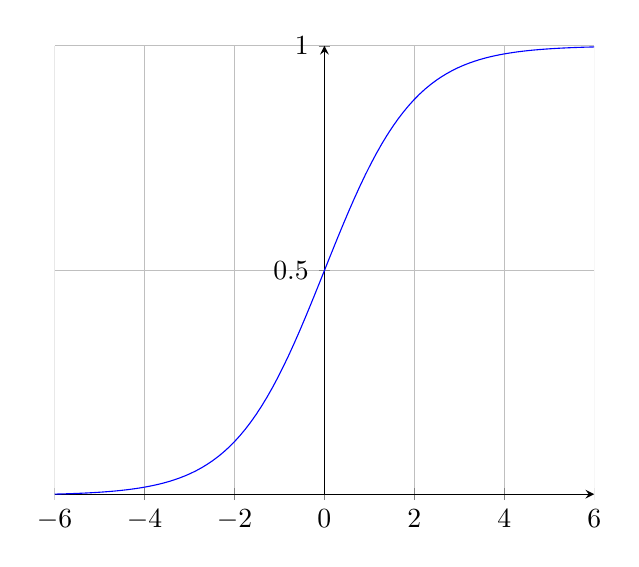
\begin{tikzpicture}
    \begin{axis}%
    [
        grid=major,     
        xmin=-6,
        xmax=6,
        axis x line=bottom,
        ytick={0,.5,1},
        ymax=1,
        axis y line=middle,
    ]
        \addplot%
        [
            blue,%
            mark=none,
            samples=100,
            domain=-6:6,
        ]
        (x,{1/(1+exp(-x))});
    \end{axis}
\end{tikzpicture}
\caption{The curve of the Sigmoid function}\label{sigmoid_curve}
\end{figure}

La régression logistique est un des modèles multivariables couramment utilisé en épidémiologie \cite{Am02,Pr05}  (c’est-à-dire l’étude de l’incidence, de la distribution et du contrôle possible des maladies et d’autres facteurs liés à des problèmes de santé pouvant affecter des groupes de population). Dans un tel contexte la variable dépendante est habituellement la survenue ou non d'un événement (maladie ou autre) et les variables indépendantes sont celles susceptibles d'influencer la survenue de cet événement c'est-à-dire les variables mesurant l'exposition à un facteur de risque ou à un facteur protecteur, ou variable représentant un facteur de confusion. L'intérêt majeur de cette technique est de quantifier la force de l'association entre chaque variable indépendante et la variable dépendante, en tenant compte de l'effet des autres variables intégrées dans le modèle \cite{Am02} .

\subsubsection{Définition fonctionnelle de notre modèle de régression.}
On supposera que la variable  \textsc{Y} à laquelle on s'intéresse est la survenue ou non du paludisme, dont les deux catégories seront notées \textsc{M+} et \textsc{M-}.
Dans le cas particulier d'une seule variable \emph{a} explicative (équivalent d'une régression simple), le modèle s'écrit :
\begin{equation}
\textsc{Pr}(\textsc{M+} ~|~ \emph{a}) = \frac{e^{\alpha + \beta\times \emph{a} }}{1 + e^{\alpha + \beta\times \emph{a} }}
\label{simple_regression}
\end{equation}
où les coefficients $\alpha$ et $\beta$ sont les paramètres du modèle.
\textsc{Pr}(\textsc{M+} ~$|$~ \emph{a})mesure la probabilité d’apparition du paludisme si la variable \emph{a} est observé. La figure \ref{courbe de la fonction sigmoide} représente la fonction logistique correspondante \emph{f(a)}. Encore une fois, l’intérêt principal de cette fonction réside dans la simplicité d’atteindre une estimation des odd ratio (OR) qui mesure la force de l'association entre la maladie \textsc{M} et une variable d'exposition dans une analyse de régression. En effet, si l'exposition est codée en $0$ (la variable n’est pas observée) et$1$ (la variable est observée) comme dans notre cas, le modèle permet d'arriver après simplification à           OR = $e^{\beta}$. Le coefficient $\beta$ de la variable d'exposition dans le modèle logistique est donc le logarithme de l'odds-ratio mesurant l'association entre cette variable (signe ou symptôme) et la maladie (paludisme), ce qui permet d'interpréter facilement les résultats d'une régression logistique.
L'extension vers un modèle à plusieurs variables (régression multiple) se fait très simplement comme le montre la formule ci-dessous
\begin{equation}
\textsc{Pr}(\textsc{M+} ~|~ \emph{$a_1$},\emph{$a_2$}, \ldots, \emph{$a_n$}) = \frac{e^{\alpha + \sum_{i=1}^{n} \beta_i \times \emph{$a_i$} }}{1 + e^{\alpha + \sum_{i=1}^{n} \beta_i \times \emph{$a_i$} }}
\label{multiple_regression}
\end{equation} 
À chaque variable\emph{$a_i$} est associé un coefficient $\beta_i$ et OR$_i$ (mesurant l'association entre Xi et M+) se calcule par  $e^{\beta_i}$.
\subsubsection{Optimisation du modèle.}La question qui se pose généralement lorsqu’on utilise une régression multiple consiste à savoir comment sélectionner l’ensemble minimal de variables parmi les \emph{$a_i$} qui explique mieux la variable \textsc{Y}. Plusieurs stratégies d’optimisation sont possibles pour obtenir le meilleur modèle de prédiction finale qui prend en compte le maximum d'informations tout en restreignant autant que possible le nombre de variables explicatives afin de faciliter l'analyse des résultats. Les plus employées sont les  procédures dites \emph{pas à pas descendantes} ou \emph{pas à pas ascendantes}. Les deux approches appliquent une régression itérative en incluant d’abord dans le modèle la variable qui présente le meilleur coefficient de détermination, puis en ajoutant la variable qui améliore ce coefficient et ainsi de suite pour les méthodes ou pas à pas ascendantes. Pour les méthodes ou pas à pas descendantes, l’ensemble des variables est considéré au début et les variables sont progressivement exclus du modèle, en fonction de ceux qui n’ont pas significativement amélioré le coefficient de détermination.
Dans la section suivante nous présentons les résultats de nos expérimentations obtenues en utilisant notre modèle de régression logistique sur des données réelles de patients











% Experimentation and Results
\section{Expérimentation et Résultats}\label{Expérimentation et Résultats}
Dans cette section, nous présentons les performances de notre modèle de prédiction  du paludisme à travers une analyse des résultats des expérimentations que nous avons menées sur des jeux de données du  réelles de patients  et un jeu de données semi-synthétique obtenue  à partir du jeu de données réelles. Nous commençons par présenter les conditions d’expérimentation
\subsection{Conditions d’expérimentations}
Nous avons testé le modèle sur trois jeux de données différents en implémentant l’algorithme de la régression logistique avec le logiciel Python. Pour imputer  les données manquantes, nous avons utilisé le package missForest du logiciel R est utilisé.

\subsubsection{Nos jeux de données.} Nous avons collecté et utilisé un jeu de données patient réels provenant de différents points de santé qui ont été définis lors du Grand Magal de Touba en 2016. Nous avons également généré et utilisé deux variantes de ce jeu de données de patient réels. La description des caractéristiques de notre jeu de données brutes de patients réels, ainsi que le processus  de préparation des données que nous avions proposées pour nettoyer, normaliser et imputer les informations, sont données dans la section \ref{data_prep}. Nous notons \textsc{DT1} ce jeu de données.
La première variante, notée \textsc{DT2} est obtenue en supprimant les enregistrements avec les attributs manquants dans \textsc{DT1} au lieu d'utiliser un algorithme d'imputation qui prédit les valeurs des informations manquantes.

Une telle variante aidera à étudier l’impact de la suppression des enregistrements avec des valeurs manquantes dans l'exactitude de la prévision.
La deuxième variante, appelée \textsc{DT3}, est un jeu de données semi-synthétique qui a été généré en utilisant une stratégie de sur échantillonnage sur le jeu  de données brutes \textsc{DT1}. En effet une analyse explicative effectuée sur le jeu de données \textsc{DT1} a révélé que les données sont assez déséquilibrés, c'est-à-dire qu'il montre un déséquilibre important entre les classes; le nombre de  patients atteints de paludisme était largement inférieur au nombre de patients qui ne souffrent pas de paludisme, comme illustré à la figure \ref{records_class}. L’exploitation des approches d'échantillonnage peut permettre d’obtenir un jeu de données équilibré concernant les deux classes à prédire. 
Pour cela nous avons implémenté l’algorithme SMOTE \cite{Wa06},  avec le package \emph{imbalanced-learn} \cite{Gu17}. SMOTE consiste à créer un échantillon de données semi synthétiques à partir de la valeur dépendante  diagnostic au lieu de faire des copies des valeurs existantes. Ensuite, choisir de manière aléatoire, l'un des k plus proches voisins et l'utiliser pour créer de nouvelles observations similaires, mais au hasard.
Dossier donné afin de créer de nouvelles observations au hasard. Nous avons appliqué un sur échantillonnage de la classe minoritaire dans notre jeu de données patient pour générer un ensemble  semi-synthétique de données \textsc{DT3} contenant le même nombre d'enregistrements pour les deux classes.
% distribution of records by class
\begin{figure}[h]
\centering
\includegraphics[width=0.6\textwidth]{images/imbalanced_dataset}
\label{records_class}\caption{The number of records by class}
\end{figure} 
% Implementation of the logistic model
\subsubsection{Paramètres du modèle de prédiction.}
 Afin de mettre en place notre modèle de classification basée sur la régression logistique, la librairie sklearn1 de Python \emph{sklearn} library\footnote{https://scikit-learn.org/stable/modules/generated/sklearn.linear\_model.LogisticRegression.html}. Ce package de python définit les paramètres par défaut de la régression logistique, ainsi que des stratégies d'optimisation, pour effectuer correctement la classification binaire en utilisant le meilleur modèle final. Pour les besoins de nos tests, nous avons utilisé les paramètres d'entrée de la régression logistique suivante
 \begin{itemize}
\item \textbf{random\_state}: modélise le l’état initial du générateur de nombres pseudo aléatoires à utiliser lors du mélange des données. Sa valeur est définie à 0 car nous n’avons pas besoin de mélanger les données dans notre expérimentation.
\item \textbf{class\_weight}: c’est le poids associés aux classes. Nous le réglons sur ‘None’, c'est-à-dire que toutes les classes sont censées avoir le poids qui est égale à 1.
\item \textbf{dual}. Il n’est mise en œuvre que pour les problèmes avec une pénalisation l2. Ce paramètre est défini sur Faux car le nombre d’échantillons est supérieur au nombre de fonctionnalités.
\item \textbf{fit\_intercept}: utile si une constante (ou biais) est ajoutée à la fonction de prédiction. Par conséquent, nous avons fixé l’interception d’ajustement à Vrai.
\item \textbf{intercept\_scaling}: ce paramètre, défini sur 1, n'est utile que lorsque le solveur «liblinear» est utilisé et fit_intercept est défini sur Vrai.
\item \textbf{max\_iter}: nombre maximum d'itérations prises pour que les solveurs convergent.
\item \textbf{multi\_class}: si l'option choisie est ovr, alors un problème binaire est correct.
\item \textbf{n\_jobs}: nombre de processeurs cpu utilisés lors de la parallélisation de classes si multi class = "ovr". Ce paramètre est ignoré lorsque le solveur est défini sur “liblinear” que «multiclass» soit spécifié ou non.

\item \textbf{penalty}: ce paramètre est utilisé pour spécifier la norme dans la pénalisation. Nous avons fixé la pénalité à sa valeur par défaut 1/2.
\item \textbf{solver}: il permet de spécifier la stratégie utilisée pour résoudre l'optimisation sous-jacente de notre modèle. Il est fixé à liblinear.
\item \textbf{tol:} tolérance pour le critère d'arrêt définie sur 0.0001.
\item \textbf{verbose}: pour le liblinear solver, définissez verbose sur un nombre positif 
\item \textbf{warm\_start}: lorsqu'il est défini sur True, réutilise la solution de l'appel précédent pour l'adapter à l'initialisation, sinon, effacez la solution précédente. Inutile pour le liblinear solver.
\end{itemize}
Comme la régression logistique effectue un apprentissage supervisé, nous avons utilisé 60\%  du jeu de données pour l’entrainement du modèle et 30\%  du jeu de données  pour  de test.



% Conclusion
\input{conclusion}

%
% ---- Bibliography ----
%
% BibTeX users should specify bibliography style 'splncs04'.
% References will then be sorted and formatted in the correct style.
%
\bibliographystyle{splncs04}
\bibliography{biblio}
%
\end{document}
